\documentclass[12pt]{article}
\usepackage[all, stdclass]{lix}
\usepackage{graphicx}
\usepackage{svg}
\svgsetup{
  inkscapepath=assets/,  % Path to the directory containing your SVG files
  svgpath=assets/        % Path to the directory containing your SVG files
}
\usepackage{float}
\usepackage{hyperref}
\usepackage{times}
\usepackage{amsmath}


%----------EDIT COVER INFO HERE -----------------%

\def \LOGOPATH {assets/birzeit-logo.png}
\def \DEPARTEMENT {Department of Electrical \& Computer Engineering}
\def \COURSENUM {ENEE2103}
\def \COURSENAME {Circuits and Electronics Laboratory}
\def \REPORTTITLE {Operational Amplifier}
\def \STUDENTNAME {Mohammad Abu-Shelbaia}
\def \STUDENTID {1200198}
\def \INSTRUCTOR {Dr. Mahran Quran}
\def \ASSISTANT {Eng. Rafah Rahhal}
\def \REPORTNUM {10}

\begin{document}
\pagenumbering{Roman}

\begin{titlepage}
    \vfill
    \begin{center}
        \includegraphics[width=0.7\textwidth]{\LOGOPATH} \\
        \hfill \\
        \Large{\DEPARTEMENT} \\
        \Large{\COURSENUM\;-\;\COURSENAME} \\
        \vfill
        \textbf{\LARGE{Experiment \#\REPORTNUM}} \\
        \textbf{\LARGE{\REPORTTITLE}}
    \end{center}
    \vfill
    \begin{flushleft}
        \Large{\textbf{Prepared by:}\\ \STUDENTNAME\quad\STUDENTID} \\

        \Large{\textbf{Instructor:} \INSTRUCTOR} \\
        \Large{\textbf{Assistant:} \ASSISTANT} \\
        \Large{\textbf{Section:} 4}\\
        \LARGE{\textbf{ }}\\
        \LARGE{\textbf{ }}\\
        \LARGE{\textbf{ }}\\
        \Large{\textbf{Date:} \today}\\
    \end{flushleft}
    \vfill
\end{titlepage}


%--------------- TABLES --------------------------------%
\tableofcontents
\clearpage
\setlength{\parskip}{\baselineskip}%
\listoffigures
\clearpage
\listoftables
\clearpage
\pagenumbering{arabic}
%-------------- CONTENT ---------------------%
\h{Simulation and Data Analysis}
\hh{Inverted Adding Amplifier}
\begin{figure}[H]
    \centering
    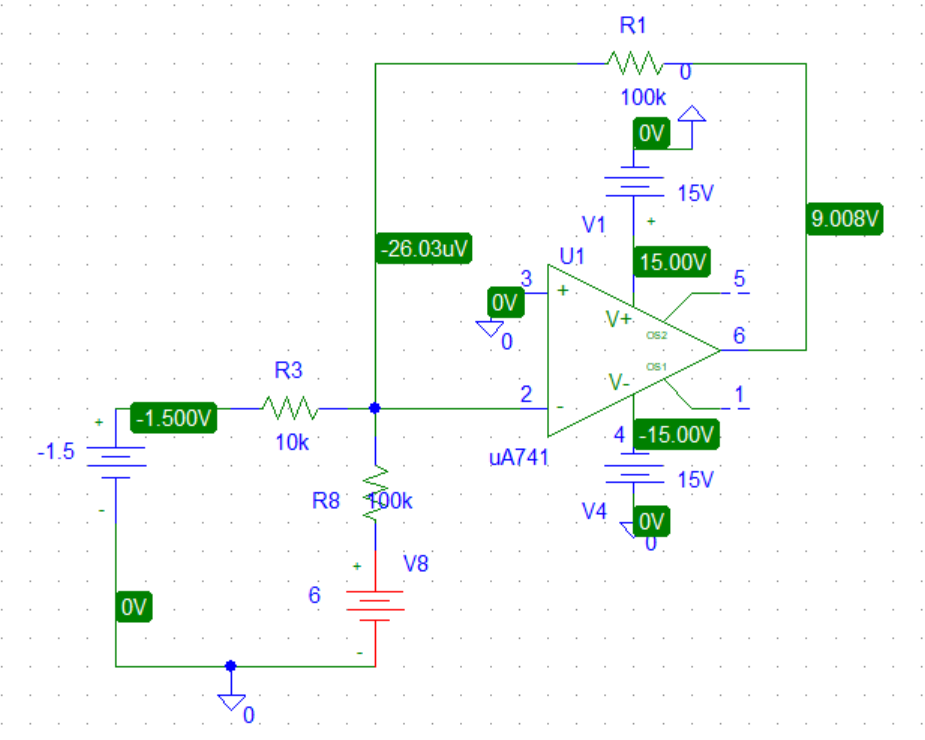
\includegraphics[width=0.5\textwidth]{assets/main/2023-08-20-13-40-43.png}
    \caption{Inverted Adder Operational Amplifier}
\end{figure}
\begin{table}[H]
    \centering
    \resizebox{0.5\textwidth}{!}{%
    \begin{tabular}{|cc|c|}
        \hline
        \multicolumn{2}{|c|}{Input Voltage} & Outoput Voltage \\ \hline
        \multicolumn{1}{|c|}{$V_1$} & $V_2$ & $V_o$           \\ \hline
        \multicolumn{1}{|c|}{0.5}   & 2     & -6.991          \\ \hline
        \multicolumn{1}{|c|}{0.3}   & 4     & -6.991          \\ \hline
        \multicolumn{1}{|c|}{-0.9}  & 2     & 7.008           \\ \hline
        \multicolumn{1}{|c|}{-1.5}  & 6     & 9.008           \\ \hline
    \end{tabular}%
    }
    \caption{Adding Amplifier Voltage Reads}
    \label{tab:my-table}
\end{table}
\begin{equation}
    V_o \approx -9.987V_1 - 0.998V_2
\end{equation}
\hh{Voltage Follower Operational Amplifier}
\begin{figure}[H]
    \centering
    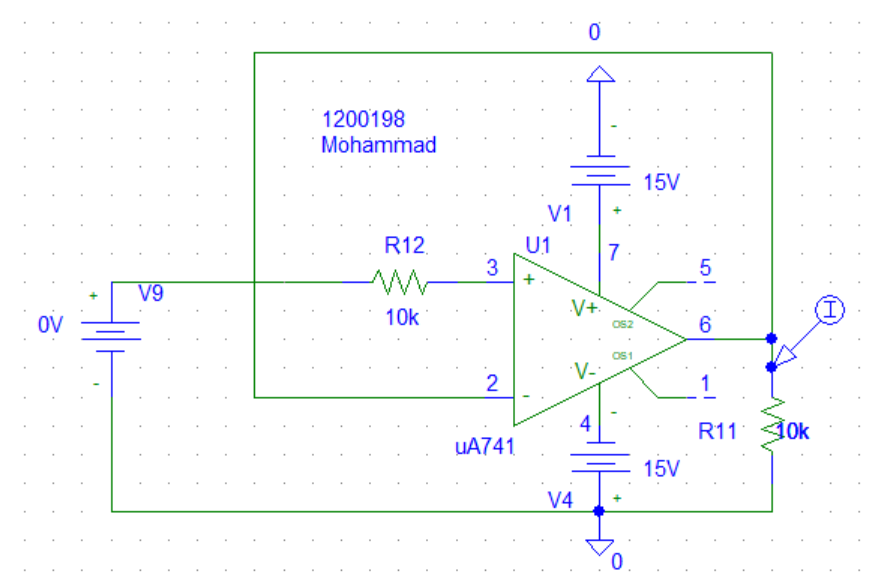
\includegraphics[width=0.5\textwidth]{assets/main/2023-08-20-14-17-05.png}
    \caption{Voltage Follower Operational Amplifier Circuit}
\end{figure}

\begin{figure}[H]
    \centering
    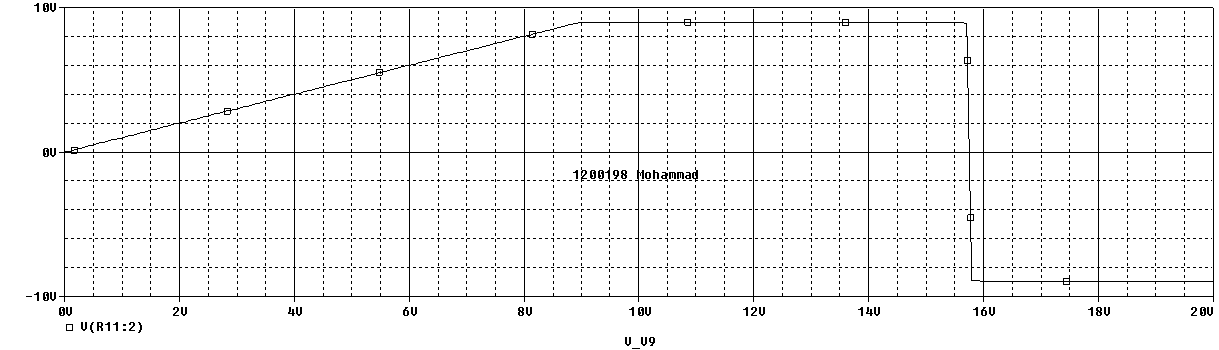
\includegraphics[width=\textwidth]{assets/main/2023-08-20-13-59-33.png}
    \caption{$V_o$ over $V_i$ for Voltage Follower}
\end{figure}
\begin{figure}[H]
    \centering
    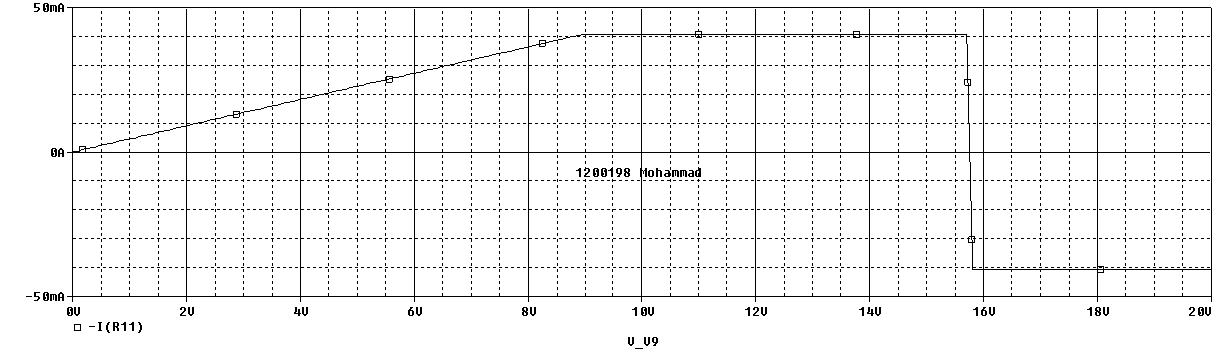
\includegraphics[width=\textwidth]{assets/main/2023-08-20-14-03-35.png}
    \caption{$I_o$ [220$\Omega$] for Voltage Follower Operational Amplifier}
\end{figure}
We can see that the current is liniearly increasing with the voltage, which is expected since the resistance is constant. But at $I_o = 40mA$ the current is constant disregarding the voltage, and after $V_i \approx 15.5V$ the current is constant at $I_o = -40mA$.
\begin{figure}[H]
    \centering
    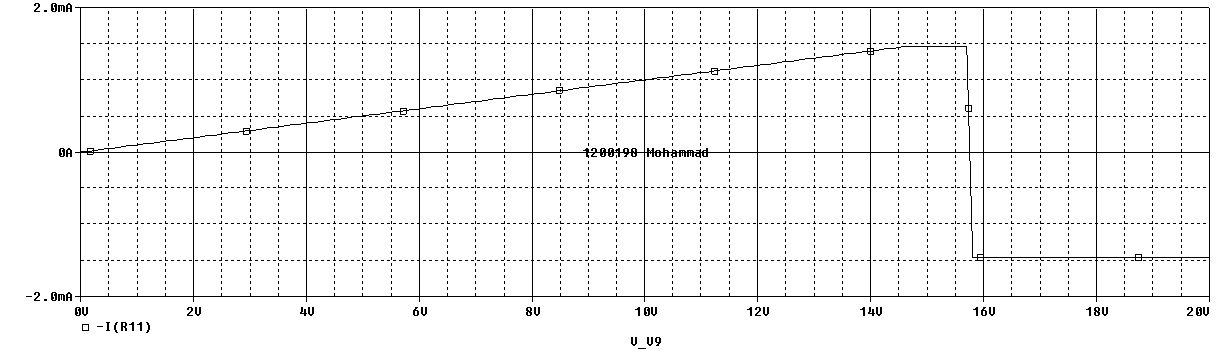
\includegraphics[width=\textwidth]{assets/main/2023-08-20-14-04-48.png}
    \caption{$I_o$ [10K$\Omega$] for Voltage Follower Operational Amplifier}
\end{figure}
We notice the same behavior as the previous circuit, but the current is constant at $I_o = 1.5mA$ and $I_o = -1.5mA$ when voltage crosses $V_i \approx 15.5V$.
\hh{Comparator Operational Amplifier}
\begin{figure}[H]
    \centering
    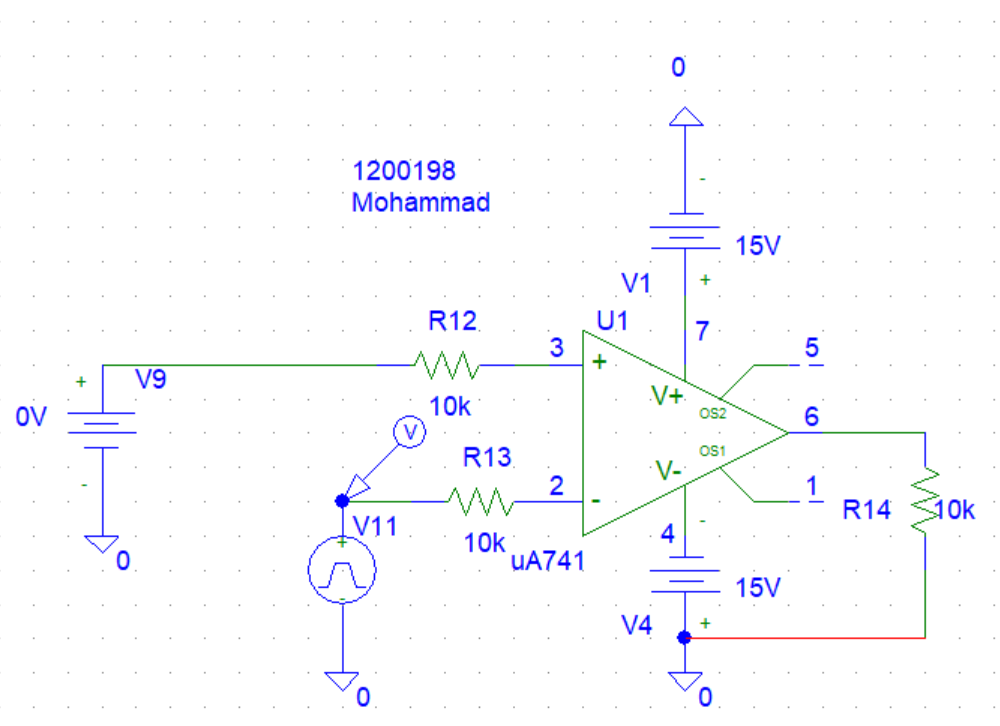
\includegraphics[width=0.5\textwidth]{assets/main/2023-08-20-14-25-10.png}
    \caption{Comparator Operational Amplifier Circuit}
\end{figure}

\begin{figure}[H]
    \centering
    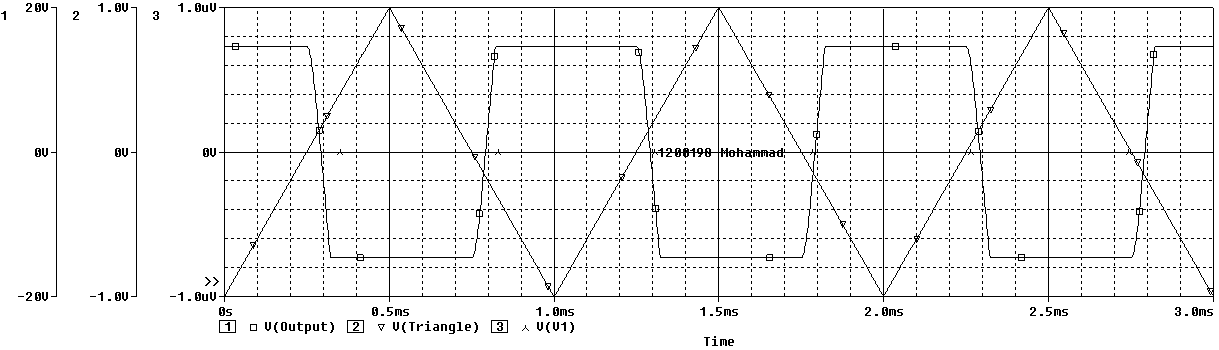
\includegraphics[width=\textwidth]{assets/main/2023-08-20-15-12-14.png}
    \caption{Comparator Operational Amplifier Output}
\end{figure}
We notice that whenever $V_1 > V_2$ the output is $V_o = 15V$, and whenever $V_1 < V_2$ the output is $V_o = -15V$.
\begin{figure}[H]
    \centering
    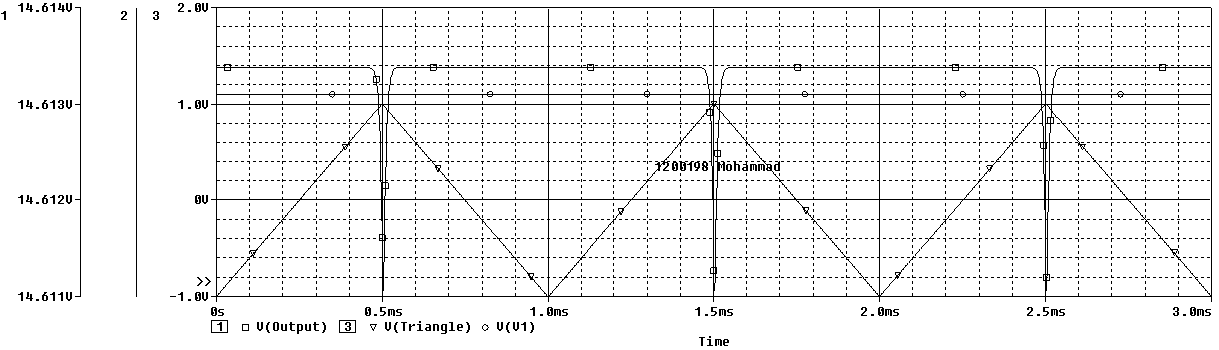
\includegraphics[width=\textwidth]{assets/main/2023-08-20-15-19-07.png}
    \caption{Comparator Operational Amplifier Output [$V_1 = 1.1V$]}
\end{figure}
From the previous graph, we can see that the output is always $V_o \approx 15V$ since $V_1 > V_2$.
\begin{figure}[H]
    \centering
    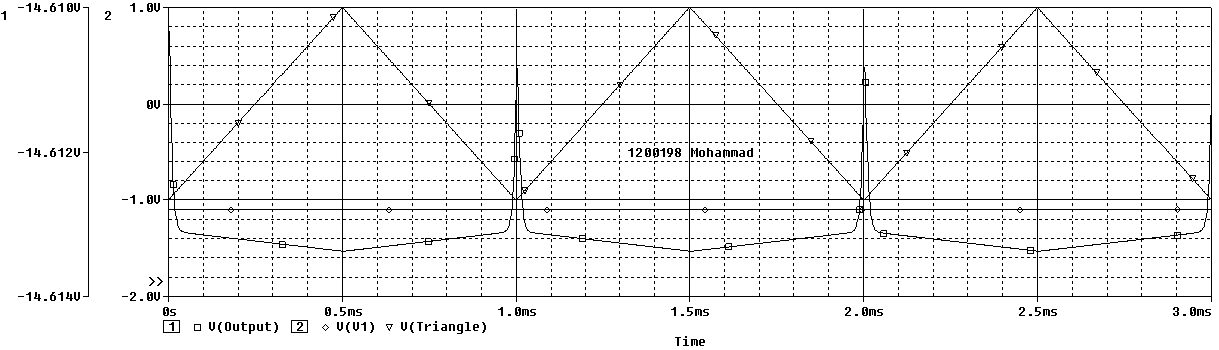
\includegraphics[width=\textwidth]{assets/main/2023-08-20-15-24-09.png}
    \caption{Comparator Operational Amplifier Output [$V_1 = 1.1V$]}
\end{figure}
From the previous graph, we can see that the output is always $V_o \approx -15V$ since $V_1 < V_2$.
\hh{Comparator with Hysteresis Operational Amplifier}
\begin{figure}[H]
    \centering
    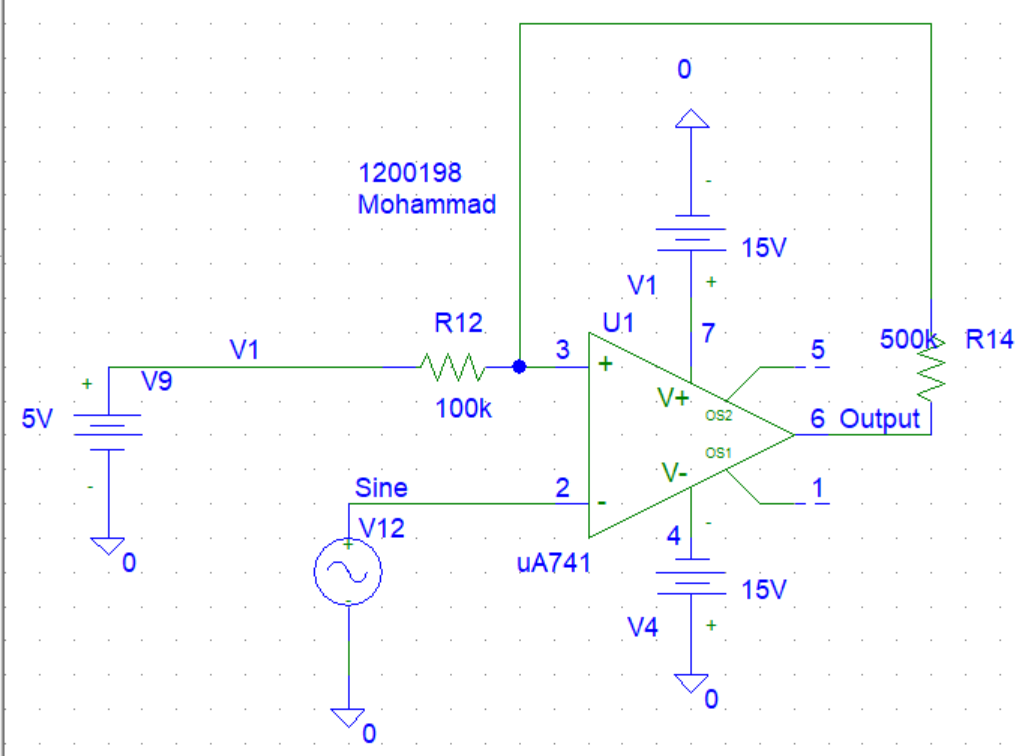
\includegraphics[width=0.5\textwidth]{assets/main/2023-08-20-15-28-53.png}
    \caption{Comparator with Hysteresis Operational Amplifier Circuit}
\end{figure}

\begin{figure}[H]
    \centering
    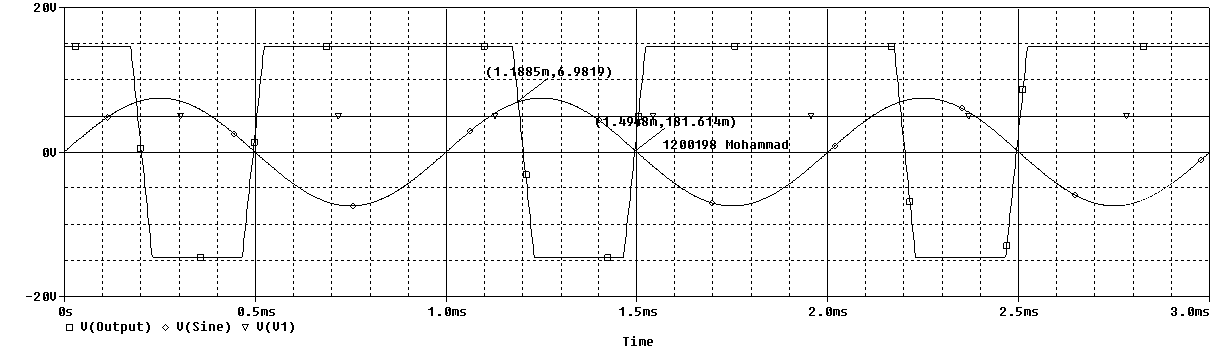
\includegraphics[width=\textwidth]{assets/main/2023-08-20-15-32-24.png}
    \caption{Comparator with Hysteresis Operational Amplifier Output}
\end{figure}
At around $V_i = 6.98V$ the output switches from $V_o = 15V$ to $V_o = -15V$, and at around $V_i = 0V$ the output switches from $V_o = -15V$ to $V_o = 15V$.
\end{document}





